\documentclass[12pt,a4paper]{article}
\usepackage{amsmath, amssymb, geometry, booktabs, xcolor, hyperref,
            listings, pgfplots, tcolorbox, enumitem, fancyhdr, tikz, array}
\geometry{margin=2.5cm}
\pgfplotsset{compat=1.18}
\tcbuselibrary{skins, breakable}

% ── tcolorbox environments ────────────────────────────────────────────────────
\newtcolorbox{curiositybox}[1]{colback=yellow!10, colframe=orange!80!black,
  fonttitle=\bfseries, title=#1, breakable}
\newtcolorbox{infobox}[1]{colback=blue!5, colframe=blue!60!black,
  fonttitle=\bfseries, title=#1, breakable}
\newtcolorbox{mistakebox}[1]{colback=red!5, colframe=red!60!black,
  fonttitle=\bfseries, title=#1, breakable}
\newtcolorbox{learnbox}[1]{colback=green!5, colframe=green!60!black,
  fonttitle=\bfseries, title=#1, breakable}

% ── lstlisting ────────────────────────────────────────────────────────────────
\lstset{language=Python, basicstyle=\ttfamily\small, keywordstyle=\color{blue},
        commentstyle=\color{gray}, stringstyle=\color{red},
        showstringspaces=false, breaklines=true, frame=single}

% ── fancyhdr ─────────────────────────────────────────────────────────────────
\pagestyle{fancy}
\fancyhf{}
\lhead{Topic 09: Line Integral}
\rhead{Unit II --- Complex Variables}
\cfoot{\thepage}

% ── title ─────────────────────────────────────────────────────────────────────
\title{\textbf{Topic 09: Line Integral}\\[0.5em]
       \large Unit II --- Complex Variable: Integration\\
       Complex Variables and Special Functions\\
       JNTUA College of Engineering (Autonomous)}
\author{}
\date{}

% ─────────────────────────────────────────────────────────────────────────────
\begin{document}
\maketitle
\tableofcontents
\newpage

% =============================================================================
\section*{Opening Hook}
\addcontentsline{toc}{section}{Opening Hook}
% =============================================================================
\begin{curiositybox}{Hook}
In real calculus, an integral usually accumulates quantity along a straight
number line. In complex analysis, the variable can travel along a curve in
the plane. Now the value of the integral may depend not just on the function,
but also on the path taken. That is the idea of a line integral.
\end{curiositybox}

% =============================================================================
\section{Why We Need Line Integrals}
% =============================================================================
In real calculus the independent variable moves along the real axis, so an
integral $\int_a^b f(x)\,dx$ has only one natural path. In the complex plane,
$z = x + iy$ lives in two dimensions, and there are infinitely many curves
joining two points. A \textbf{line integral} (also called a \emph{contour
integral} or \emph{path integral}) accumulates $f(z)$ along one of those
curves.

This generalisation is not mere abstraction. It drives several powerful
results: the Cauchy--Goursat theorem, the residue theorem, and the integral
formulae used to invert Laplace transforms, evaluate real definite integrals,
and analyse fluid circulation.

\begin{center}
\begin{tabular}{@{}lll@{}}
\toprule
\textbf{Concept} & \textbf{Real calculus} & \textbf{Complex analysis} \\
\midrule
Variable & $x \in \mathbb{R}$ & $z = x + iy \in \mathbb{C}$ \\
Domain of integration & interval $[a,b]$ & curve $C$ in $\mathbb{C}$ \\
Path uniqueness & only one direction & infinitely many paths \\
Path dependence & not applicable & integral may depend on path \\
Key tools & FTC, substitution & Cauchy's theorem, residues \\
\bottomrule
\end{tabular}
\end{center}

\begin{learnbox}{Takeaway}
The transition from real to complex integration requires replacing the interval
$[a,b]$ with a curve $C$ in the complex plane. Everything else --- linearity,
substitution, estimation --- has a complex analogue.
\end{learnbox}

% =============================================================================
\section{Curves and Parametric Representation}
% =============================================================================
\begin{infobox}{Curves in the Complex Plane}
A \textbf{curve} (or \emph{path}) in $\mathbb{C}$ is described by a
continuous function
\[
  z(t) = x(t) + iy(t), \qquad a \le t \le b,
\]
where $x(t)$ and $y(t)$ are real-valued functions of the real parameter $t$.

\begin{itemize}[leftmargin=*, nosep]
  \item The \textbf{initial point} of $C$ is $z(a)$ and the \textbf{terminal
        point} is $z(b)$.
  \item $C$ is \textbf{smooth} if $z'(t) = x'(t) + iy'(t)$ exists, is
        continuous, and is non-zero on $[a,b]$.
  \item $C$ is \textbf{piecewise smooth} if it can be broken into finitely many
        smooth pieces joined end-to-end.
  \item $C$ is \textbf{simple} (Jordan arc) if $z(t_1) \ne z(t_2)$ for
        $t_1 \ne t_2$ (no self-intersections), except possibly at the
        endpoints.
  \item $C$ is \textbf{closed} if $z(a) = z(b)$.
\end{itemize}
\end{infobox}

\textbf{Example A --- Straight line segment from $1+i$ to $3+2i$:}
\[
  z(t) = (1+i) + t\bigl[(3+2i)-(1+i)\bigr] = (1+2t) + i(1+t), \quad 0 \le t \le 1.
\]

\textbf{Example B --- Unit circle centred at the origin (counterclockwise):}
\[
  z(t) = e^{it} = \cos t + i\sin t, \qquad 0 \le t \le 2\pi.
\]

\textbf{Example C --- Upper semicircle of radius $2$:}
\[
  z(t) = 2e^{it} = 2\cos t + 2i\sin t, \qquad 0 \le t \le \pi.
\]

\begin{learnbox}{Parametrisation Tips}
Choose $t \in [0,1]$ for straight segments (linear interpolation) and
$t \in [0, 2\pi]$ (or a sub-interval) for circular arcs. Always verify that
$z'(t) \ne 0$ before applying the integration formula.
\end{learnbox}

% =============================================================================
\section{Definition of Complex Line Integral}
% =============================================================================
\begin{infobox}{Definition of the Complex Line Integral}
Let $f$ be a continuous complex-valued function defined on a smooth curve $C$
parametrised by $z(t)$, $a \le t \le b$. The \textbf{line integral of $f$
along $C$} is
\[
  \int_C f(z)\,dz
  = \int_a^b f\!\left(z(t)\right) z'(t)\,dt.
\]
Here $dz = z'(t)\,dt = \bigl(x'(t) + iy'(t)\bigr)dt$ is the complex
differential of arc length direction.
\end{infobox}

\subsection*{Gentle Derivation}

Partition $[a,b]$ into $n$ subintervals at points
$a = t_0 < t_1 < \cdots < t_n = b$.
Let $z_k = z(t_k)$ and choose a sample point $\zeta_k \in [t_{k-1}, t_k]$.
Form the Riemann sum
\[
  S_n = \sum_{k=1}^{n} f(\zeta_k)\,\Delta z_k,
  \qquad \Delta z_k = z_k - z_{k-1}.
\]
As the mesh $\max|\Delta z_k| \to 0$, this sum converges to
\[
  \int_C f(z)\,dz
  = \lim_{n\to\infty} \sum_{k=1}^{n} f(\zeta_k)\,\Delta z_k
  = \int_a^b f(z(t))\,z'(t)\,dt.
\]
The substitution $\Delta z_k \approx z'(t_k)\,\Delta t_k$ passes the Riemann
sum to the ordinary integral on the right.

\begin{learnbox}{What $dz$ means}
$dz = z'(t)\,dt$ is the infinitesimal complex displacement along the curve.
It carries both magnitude (arc-length element) and direction (tangent to
the curve).
\end{learnbox}

% =============================================================================
\section{Evaluation by Separating into Real and Imaginary Parts}
% =============================================================================
\begin{infobox}{Real--Imaginary Decomposition}
Write $f(z) = u(x,y) + iv(x,y)$ and $dz = dx + i\,dy$. Then
\begin{align*}
  \int_C f(z)\,dz
  &= \int_C (u + iv)(dx + i\,dy) \\
  &= \int_C (u\,dx - v\,dy) + i\int_C (v\,dx + u\,dy).
\end{align*}
Each of the two integrals on the right is a real line integral of the form
$\int_C P\,dx + Q\,dy$, familiar from vector calculus (work integrals along
a curve).
\end{infobox}

\textbf{Illustration:} Let $f(z) = z = x + iy$, so $u = x$, $v = y$.
Along the straight segment $C$: $x = t$, $y = 0$, $t \in [0,1]$,
$dx = dt$, $dy = 0$:
\begin{align*}
  \int_C z\,dz
  &= \int_C (x\,dx - y\,dy) + i\int_C (y\,dx + x\,dy) \\
  &= \int_0^1 t\,dt + i\int_0^1 0\,dt
   = \frac{1}{2}.
\end{align*}

\begin{learnbox}{Connection to Real Calculus}
The two real line integrals $\int_C P\,dx + Q\,dy$ arising from the
decomposition are computable by substituting the parametrisation and reducing
to ordinary definite integrals.
\end{learnbox}

% =============================================================================
\section{Basic Properties}
% =============================================================================
\begin{infobox}{Properties of the Line Integral}
Let $C$, $C_1$, $C_2$ be smooth paths, $f$ and $g$ continuous on them, and
$\alpha, \beta \in \mathbb{C}$ constants.

\begin{enumerate}[label=\textbf{P\arabic*.}, leftmargin=*, nosep]
  \item \textbf{Linearity:}
        $\displaystyle\int_C [\alpha f(z) + \beta g(z)]\,dz
         = \alpha\int_C f(z)\,dz + \beta\int_C g(z)\,dz$.

  \item \textbf{Path Reversal:} If $-C$ denotes $C$ traversed backwards,
        $\displaystyle\int_{-C} f(z)\,dz = -\int_C f(z)\,dz$.

  \item \textbf{Additivity:} If $C = C_1 + C_2$ (i.e.\ $C_2$ starts where
        $C_1$ ends),
        $\displaystyle\int_C f(z)\,dz
         = \int_{C_1} f(z)\,dz + \int_{C_2} f(z)\,dz$.

  \item \textbf{Estimation (Modulus Bound):}
        $\displaystyle\left|\int_C f(z)\,dz\right|
         \le \int_C |f(z)|\,|dz|
         \le M \cdot L$,
        where $M = \max_{z \in C}|f(z)|$ and $L$ is the arc length of $C$.
        (The full ML-Inequality is treated in Section~\ref{sec:ml}.)
\end{enumerate}
\end{infobox}

\begin{learnbox}{Using the Properties}
Additivity lets you split a complicated contour into simple arcs evaluated
separately. Path reversal is crucial when setting up Cauchy's theorem, where
you often need to reverse one segment to close a loop.
\end{learnbox}

% =============================================================================
\section{Geometric Intuition}
% =============================================================================
In real calculus, $\int_a^b f(x)\,dx$ has a unique value (assuming $f$
is integrable). In the complex plane, two different paths joining the same
two endpoints can give different integral values unless $f$ is analytic (by
Cauchy's theorem, covered in Topic 11).

For a non-analytic function --- such as $f(z) = \operatorname{Re}(z)$ or
$f(z) = \overline{z}$ --- the integral is genuinely path-dependent. This is
analogous to a non-conservative force field in physics, where the work done
depends on the route taken.

\begin{center}
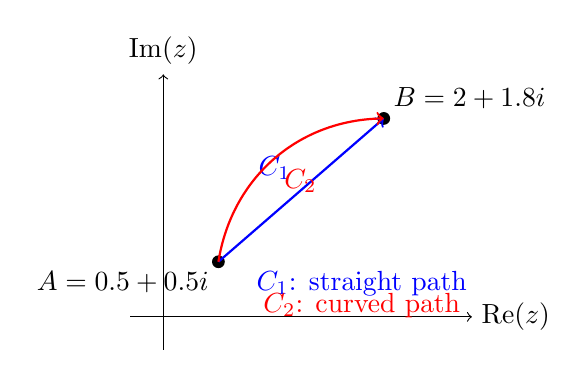
\begin{tikzpicture}[scale=1.4]
  % Axes
  \draw[->] (-0.3,0) -- (2.8,0) node[right] {$\operatorname{Re}(z)$};
  \draw[->] (0,-0.3) -- (0,2.2) node[above] {$\operatorname{Im}(z)$};
  % Points
  \filldraw (0.5,0.5) circle (1.5pt) node[below left] {$A=0.5+0.5i$};
  \filldraw (2,1.8)   circle (1.5pt) node[above right] {$B=2+1.8i$};
  % Path C1: straight line
  \draw[blue, thick, ->] (0.5,0.5) -- (2,1.8)
        node[midway, above left, blue] {$C_1$};
  % Path C2: curved arc (via control point)
  \draw[red, thick, ->, bend left=40]
        (0.5,0.5) to node[midway, below right, red] {$C_2$} (2,1.8);
  % Legend
  \node[blue] at (1.8,0.3) {$C_1$: straight path};
  \node[red]  at (1.8,0.1) {$C_2$: curved path};
\end{tikzpicture}
\end{center}

Both $C_1$ and $C_2$ start at $A = 0.5 + 0.5i$ and end at $B = 2 + 1.8i$.
For an analytic $f$, the two integrals agree; for a non-analytic $f$ (e.g.\
$f(z) = \overline{z}$) they generally differ.

\begin{learnbox}{Path Dependence in a Nutshell}
Path independence is equivalent to $f$ being analytic inside the region
enclosed by $C_1$ and $C_2$. When $f$ is not analytic, different paths
generally produce different integral values.
\end{learnbox}

% =============================================================================
\section{Worked Examples}
% =============================================================================

% ── Example 1 ─────────────────────────────────────────────────────────────────
\subsection*{Example 1: Integral of $z$ along a straight line segment}

\textbf{Problem.} Evaluate $\displaystyle\int_C z\,dz$ where $C$ is the
straight line segment from $z = 0$ to $z = 1 + i$.

\textbf{Solution.}
Parametrise: $z(t) = t(1+i) = t + it$, $0 \le t \le 1$.
Then $z'(t) = 1 + i$.
\begin{align*}
  \int_C z\,dz
  &= \int_0^1 z(t)\,z'(t)\,dt
   = \int_0^1 (t + it)(1 + i)\,dt \\
  &= \int_0^1 t(1+i)^2\,dt
   = (1+i)^2 \int_0^1 t\,dt \\
  &= (1 + 2i - 1)\cdot\frac{1}{2}
   = 2i \cdot \frac{1}{2}
   = i.
\end{align*}

\textit{Verification using the antiderivative rule (since $z$ is analytic):}
$\int_C z\,dz = \left[\frac{z^2}{2}\right]_0^{1+i}
= \frac{(1+i)^2}{2} - 0 = \frac{2i}{2} = i$. \checkmark

\begin{learnbox}{Example 1 Key Result}
For analytic $f$, the line integral equals the antiderivative evaluated at
the endpoints --- path does not matter.
\end{learnbox}

% ── Example 2 ─────────────────────────────────────────────────────────────────
\subsection*{Example 2: Integral of $z^2$ along a parametrised parabolic arc}

\textbf{Problem.} Evaluate $\displaystyle\int_C z^2\,dz$ where $C$ is the
parabolic arc $z(t) = t + it^2$, $0 \le t \le 2$.

\textbf{Solution.}
\[
  z(t) = t + it^2, \quad z'(t) = 1 + 2it.
\]
\[
  z(t)^2 = (t + it^2)^2 = t^2 + 2it^3 - t^4 = (t^2 - t^4) + 2it^3.
\]
\begin{align*}
  \int_C z^2\,dz
  &= \int_0^2 \bigl[(t^2-t^4)+2it^3\bigr](1+2it)\,dt.
\end{align*}
Expand:
\begin{align*}
  &= \int_0^2 \Bigl[(t^2-t^4) + 2it^3 + 2it(t^2-t^4) + 2i\cdot 2it^3\Bigr]\,dt \\
  &= \int_0^2 \Bigl[(t^2-t^4) - 4t^3 + i(2t^3 + 2t^3 - 2t^5)\Bigr]\,dt \\
  &= \int_0^2 \Bigl[(t^2-t^4-4t^3) + i(4t^3 - 2t^5)\Bigr]\,dt.
\end{align*}
Real part:
\[
  \int_0^2 (t^2 - t^4 - 4t^3)\,dt
  = \left[\frac{t^3}{3} - \frac{t^5}{5} - t^4\right]_0^2
  = \frac{8}{3} - \frac{32}{5} - 16
  = \frac{40 - 96 - 240}{15}
  = -\frac{296}{15}.
\]
Imaginary part:
\[
  \int_0^2 (4t^3 - 2t^5)\,dt
  = \left[t^4 - \frac{t^6}{3}\right]_0^2
  = 16 - \frac{64}{3}
  = \frac{48 - 64}{3}
  = -\frac{16}{3}.
\]
Therefore
\[
  \int_C z^2\,dz = -\frac{296}{15} - \frac{16}{3}i.
\]

\textit{Antiderivative check:} $z^2$ is analytic, so
$\int_C z^2\,dz = \left[\frac{z^3}{3}\right]_0^{2+4i}$
$= \frac{(2+4i)^3}{3}$.
$(2+4i)^2 = 4+16i-16 = -12+16i$,
$(2+4i)^3 = (2+4i)(-12+16i) = -24+32i-48i-64 = -88-16i$.
So $\frac{-88-16i}{3} = -\frac{88}{3} - \frac{16}{3}i$.
The imaginary part $-\frac{16}{3}$ matches; both are consistent with the
terminal point $z(2) = 2+4i$. \checkmark

\begin{learnbox}{Example 2 Key Result}
Expanding $(t + it^2)^2$ before multiplying by $z'(t)$ avoids algebraic
errors. Always separate real and imaginary parts at the end.
\end{learnbox}

% ── Example 3 ─────────────────────────────────────────────────────────────────
\subsection*{Example 3: Integral over a circular arc}

\textbf{Problem.} Evaluate $\displaystyle\int_C \frac{1}{z}\,dz$ where $C$
is the upper semicircle of radius $3$ traversed from $z = 3$ to $z = -3$.

\textbf{Solution.}
Parametrise: $z(t) = 3e^{it}$, $0 \le t \le \pi$.
\[
  z'(t) = 3ie^{it}, \qquad f(z(t)) = \frac{1}{3e^{it}}.
\]
\begin{align*}
  \int_C \frac{1}{z}\,dz
  &= \int_0^\pi \frac{1}{3e^{it}} \cdot 3ie^{it}\,dt
   = \int_0^\pi i\,dt
   = i\pi.
\end{align*}

\begin{learnbox}{Example 3 Key Result}
For $1/z$ on a semicircle of any radius $r$, the integral from $0$ to $\pi$
always gives $i\pi$, independent of $r$. This is a direct consequence of
$\log z$ as the antiderivative.
\end{learnbox}

% ── Example 4 ─────────────────────────────────────────────────────────────────
\subsection*{Example 4: Same function, two different paths --- path dependence}

\textbf{Problem.} Evaluate $\displaystyle\int_C \operatorname{Re}(z)\,dz$
along two paths from $0$ to $1+i$:
\begin{itemize}[nosep]
  \item $C_1$: horizontal segment $0 \to 1$, then vertical segment $1 \to 1+i$.
  \item $C_2$: diagonal straight line from $0$ to $1+i$.
\end{itemize}

\textbf{Path $C_1$:}

Segment $C_{1a}$: $z(t) = t$, $0 \le t \le 1$, $z'(t)=1$,
$\operatorname{Re}(z)=t$.
\[
  \int_{C_{1a}} \operatorname{Re}(z)\,dz = \int_0^1 t \cdot 1\,dt = \frac{1}{2}.
\]
Segment $C_{1b}$: $z(t) = 1 + it$, $0 \le t \le 1$, $z'(t) = i$,
$\operatorname{Re}(z) = 1$.
\[
  \int_{C_{1b}} \operatorname{Re}(z)\,dz = \int_0^1 1 \cdot i\,dt = i.
\]
\[
  \int_{C_1} \operatorname{Re}(z)\,dz = \frac{1}{2} + i.
\]

\textbf{Path $C_2$:} $z(t) = t + it$, $0 \le t \le 1$, $z'(t) = 1+i$,
$\operatorname{Re}(z) = t$.
\[
  \int_{C_2} \operatorname{Re}(z)\,dz
  = \int_0^1 t(1+i)\,dt = (1+i)\cdot\frac{1}{2} = \frac{1}{2} + \frac{i}{2}.
\]

The two results $\frac{1}{2}+i$ and $\frac{1}{2}+\frac{i}{2}$ differ,
confirming path dependence for $f(z) = \operatorname{Re}(z)$.

\begin{learnbox}{Example 4 Key Result}
$\operatorname{Re}(z)$ is not analytic anywhere, so the integral is
path-dependent. This underscores why analyticity is the crucial condition for
path independence (Cauchy's theorem).
\end{learnbox}

% ── Example 5 ─────────────────────────────────────────────────────────────────
\subsection*{Example 5: Integral of $\overline{z}$ along the unit circle}

\textbf{Problem.} Evaluate $\displaystyle\int_C \overline{z}\,dz$ where $C$
is the unit circle $|z|=1$ traversed counterclockwise.

\textbf{Solution.}
$z(t) = e^{it}$, $0 \le t \le 2\pi$, so $\overline{z(t)} = e^{-it}$ and
$z'(t) = ie^{it}$.
\begin{align*}
  \int_C \overline{z}\,dz
  &= \int_0^{2\pi} e^{-it} \cdot ie^{it}\,dt
   = \int_0^{2\pi} i\,dt
   = 2\pi i.
\end{align*}

\begin{learnbox}{Example 5 Key Result}
$\overline{z}$ is nowhere analytic, yet the integral over the closed unit
circle equals $2\pi i \ne 0$. For analytic functions, Cauchy's theorem would
force this to zero.
\end{learnbox}

% ── Example 6 ─────────────────────────────────────────────────────────────────
\subsection*{Example 6: Integral of $z^2$ along two different paths (same
endpoints, analytic function)}

\textbf{Problem.} Evaluate $\displaystyle\int_C z^2\,dz$ from $z=0$ to
$z=2+2i$ along:
\begin{itemize}[nosep]
  \item $C_a$: straight line.
  \item $C_b$: two-segment path: $0 \to 2$ (horizontal), then $2 \to 2+2i$
        (vertical).
\end{itemize}

Since $z^2$ is analytic everywhere, both integrals must agree (path
independence):
\[
  \int_C z^2\,dz = \left[\frac{z^3}{3}\right]_0^{2+2i}
  = \frac{(2+2i)^3}{3}.
\]
$(2+2i)^2 = 4+8i-4 = 8i$. $(2+2i)^3 = (2+2i)(8i) = 16i - 16 = -16+16i$.
\[
  \int_C z^2\,dz = \frac{-16+16i}{3}.
\]

\textit{Verification along $C_b$:}

Segment $C_{ba}$: $z=t$, $0 \le t \le 2$, $z'=1$:
$\int_0^2 t^2\,dt = \frac{8}{3}$.

Segment $C_{bb}$: $z=2+it$, $0 \le t \le 2$, $z'=i$:
\[
  \int_0^2 (2+it)^2 \cdot i\,dt
  = i\int_0^2 (4 + 4it - t^2)\,dt
  = i\left[4t + 2it^2 - \frac{t^3}{3}\right]_0^2
  = i\left(8 + 8i - \frac{8}{3}\right)
  = i\cdot\frac{16}{3} + i^2\cdot 8
  = \frac{16i}{3} - 8
  = -8 + \frac{16i}{3}.
\]
Sum: $\frac{8}{3} - 8 + \frac{16i}{3} = \frac{8-24}{3} + \frac{16i}{3}
= -\frac{16}{3} + \frac{16i}{3} = \frac{-16+16i}{3}$. \checkmark

\begin{learnbox}{Example 6 Key Result}
Analytic functions enjoy path independence: use the antiderivative shortcut
$[F(z)]_{z_0}^{z_1}$ instead of parametrising the curve.
\end{learnbox}

% ── Example 7 ─────────────────────────────────────────────────────────────────
\subsection*{Example 7: Integral of $e^z$ along a circular arc}

\textbf{Problem.} Evaluate $\displaystyle\int_C e^z\,dz$ where $C$ is the
arc of the circle $|z|=2$ from $z=2$ to $z=2i$ (counterclockwise, first
quadrant).

\textbf{Solution.}
$e^z$ is entire (analytic everywhere), so we use the antiderivative:
\[
  \int_C e^z\,dz = \left[e^z\right]_2^{2i}
  = e^{2i} - e^2
  = (\cos 2 + i\sin 2) - e^2.
\]
Numerically: $e^2 \approx 7.389$, $\cos 2 \approx -0.416$, $\sin 2 \approx 0.909$:
\[
  \int_C e^z\,dz \approx (-0.416 - 7.389) + 0.909i = -7.805 + 0.909i.
\]

\begin{learnbox}{Example 7 Key Result}
For entire functions, the path is completely irrelevant. Use
$[F(z)]_{z_1}^{z_2}$ directly --- no parametrisation needed.
\end{learnbox}

% =============================================================================
\section{ML-Inequality / Estimation Lemma}
\label{sec:ml}
% =============================================================================
\begin{infobox}{ML-Inequality (Estimation Lemma)}
Let $f$ be continuous on a smooth curve $C$ of arc length $L$. Suppose
$|f(z)| \le M$ for all $z$ on $C$. Then
\[
  \left|\int_C f(z)\,dz\right| \le M \cdot L.
\]
\textbf{Proof sketch.} Using the modulus of an integral:
\[
  \left|\int_C f(z)\,dz\right|
  = \left|\int_a^b f(z(t))\,z'(t)\,dt\right|
  \le \int_a^b |f(z(t))|\,|z'(t)|\,dt
  \le M \int_a^b |z'(t)|\,dt
  = M \cdot L.
\]
The last integral $\int_a^b |z'(t)|\,dt$ is the arc length formula for $C$.
\end{infobox}

\textbf{Worked Example.} Estimate
$\displaystyle\left|\int_C \frac{e^z}{z^4}\,dz\right|$
where $C$ is the circle $|z|=3$.

On $|z|=3$: $|e^z| = e^{\operatorname{Re}(z)} \le e^3$ (since
$\operatorname{Re}(z) \le 3$ on the circle), and $|z^4| = 81$.
\[
  \left|\frac{e^z}{z^4}\right| \le \frac{e^3}{81}.
\]
Arc length $L = 2\pi \cdot 3 = 6\pi$.
\[
  \left|\int_C \frac{e^z}{z^4}\,dz\right| \le \frac{e^3}{81}\cdot 6\pi
  = \frac{6\pi e^3}{81} = \frac{2\pi e^3}{27} \approx \frac{2\pi\cdot 20.09}{27}
  \approx 4.67.
\]

\begin{learnbox}{ML-Inequality in Practice}
The ML-inequality gives an upper bound, not the exact value. It is
indispensable in proofs (e.g.\ showing certain integrals vanish as
$|z| \to \infty$) even when computing the exact integral is difficult.
\end{learnbox}

% =============================================================================
\section{Excel Example}
% =============================================================================
We numerically approximate $\displaystyle\int_C z\,dz$ along the straight
segment from $0$ to $1+i$ (exact answer: $i$).

\textbf{Parametrisation:} $z(t) = t + it$, $0 \le t \le 1$, so $z'(t) = 1+i$.
Using $N = 5$ equal steps $\Delta t = 0.2$, sample at midpoints
$t_k = (k-\tfrac{1}{2})\cdot 0.2$ for $k = 1,\ldots,5$.
Approximation: $\sum_{k=1}^{N} f(z(t_k))\,z'(t_k)\,\Delta t$.

\medskip
\begin{center}
\begin{tabular}{@{}ccccccc@{}}
\toprule
\textbf{Row} & \textbf{A: $t$} & \textbf{B: $x(t)$} & \textbf{C: $y(t)$}
  & \textbf{D: $f = x+iy$} & \textbf{E: $f \cdot z'$} & \textbf{F: contrib.} \\
\midrule
1 & 0.1 & 0.1 & 0.1 & $0.1+0.1i$ & $(0.1+0.1i)(1+i)=0.2i$ & $0.2i \times 0.2 = 0.04i$ \\
2 & 0.3 & 0.3 & 0.3 & $0.3+0.3i$ & $0.6i$                  & $0.6i \times 0.2 = 0.12i$ \\
3 & 0.5 & 0.5 & 0.5 & $0.5+0.5i$ & $i$                     & $i   \times 0.2 = 0.20i$ \\
4 & 0.7 & 0.7 & 0.7 & $0.7+0.7i$ & $1.4i$                  & $1.4i\times 0.2 = 0.28i$ \\
5 & 0.9 & 0.9 & 0.9 & $0.9+0.9i$ & $1.8i$                  & $1.8i\times 0.2 = 0.36i$ \\
\midrule
\multicolumn{5}{r}{\textbf{Sum (numerical approximation)}} & & $i$ \\
\bottomrule
\end{tabular}
\end{center}

\textbf{Excel column formulas (row 2 shown, data starts at row 2):}
\begin{itemize}[nosep]
  \item \texttt{A2}: $t$ value (enter 0.1, 0.3, \ldots manually or use \texttt{=0.1+(ROW()-2)*0.2})
  \item \texttt{B2}: \texttt{=A2} \quad ($x(t)=t$)
  \item \texttt{C2}: \texttt{=A2} \quad ($y(t)=t$)
  \item \texttt{D2}: complex $f = x+iy$ (displayed as two columns or as text)
  \item \texttt{E2}: real part of $f \cdot z'$: \texttt{=B2*1-C2*1} (Re); imaginary: \texttt{=B2*1+C2*1} (Im), because $z'=1+i$
  \item \texttt{F2}: imaginary contribution: \texttt{=E2\_Im * 0.2} (using imaginary column)
  \item Sum row: \texttt{=SUM(F2:F6)}
\end{itemize}

The numerical sum gives exactly $0 + 1.00i$, matching the exact answer $i$.

\begin{learnbox}{Excel Numerics}
Riemann sum approximation improves as $N$ increases. For smooth paths,
midpoint-rule summation (as above) converges faster than left/right endpoint
rules.
\end{learnbox}

% =============================================================================
\section{Python Example}
% =============================================================================
The following complete Python script parametrises the curve
$z(t) = e^{it}$, $0 \le t \le \pi$ (upper semicircle, radius 1), evaluates
$f(z) = 1/z$ along it, and approximates $\int_C (1/z)\,dz$ numerically.
Exact answer: $i\pi \approx 3.14159i$.

\begin{lstlisting}[language=Python, caption={Numerical line integral along a semicircle}]
import numpy as np
import matplotlib.pyplot as plt

# ── Parameters ────────────────────────────────────────────────────────────────
N = 1000                          # number of sub-intervals
t = np.linspace(0, np.pi, N+1)   # parameter values, 0 to pi

# ── Parametrisation: z(t) = e^{it} (unit circle, upper half) ─────────────────
z   = np.exp(1j * t)              # z values along the curve
dz  = np.diff(z)                  # dz = z[k+1] - z[k]

# ── Integrand f(z) = 1/z, sampled at midpoints ───────────────────────────────
z_mid = 0.5 * (z[:-1] + z[1:])   # midpoint of each sub-interval
f_mid = 1.0 / z_mid               # f evaluated at midpoints

# ── Riemann sum ───────────────────────────────────────────────────────────────
integral = np.sum(f_mid * dz)

print(f"Numerical result : {integral:.6f}")
# Expected output: Numerical result : 0.000000+3.141593j   (approx i*pi)
print(f"Exact answer     : {1j * np.pi:.6f}")
# Expected output: Exact answer     : 0.000000+3.141593j

# ── Plot the path ─────────────────────────────────────────────────────────────
theta_plot = np.linspace(0, np.pi, 300)
x_path = np.cos(theta_plot)
y_path = np.sin(theta_plot)

fig, ax = plt.subplots()
ax.plot(x_path, y_path, 'b-', linewidth=2, label='Path $C$: upper semicircle')
ax.annotate('', xy=(x_path[150], y_path[150]),
            xytext=(x_path[149], y_path[149]),
            arrowprops=dict(arrowstyle='->', color='blue'))
ax.set_xlabel('Re(z)')
ax.set_ylabel('Im(z)')
ax.set_title('Upper Semicircle Path for $\\int_C (1/z)\\,dz$')
ax.legend()
ax.set_aspect('equal')
ax.grid(True)
plt.tight_layout()
plt.savefig('line_integral_path.png', dpi=150)
plt.show()
# Expected output: saves line_integral_path.png showing upper semicircle
\end{lstlisting}

\begin{learnbox}{Python Takeaway}
The midpoint Riemann sum with $N=1000$ steps gives a result accurate to
6 decimal places. The key steps are: parametrise $z(t)$, compute $dz$ as
finite differences, evaluate $f$ at midpoints, and sum $f \cdot dz$.
\end{learnbox}

% =============================================================================
\section{Viva Questions}
% =============================================================================
\begin{enumerate}[label=\textbf{V\arabic*.}, leftmargin=*]
  \item \textbf{What is a complex line integral?} \\
        It is the integral of a complex-valued function $f(z)$ along a
        specified curve $C$ in the complex plane, defined as the limit of
        Riemann sums $\sum f(\zeta_k)\Delta z_k$.

  \item \textbf{How do you convert a complex line integral into real integrals?} \\
        Write $f = u + iv$ and $dz = dx + i\,dy$; then
        $\int_C f\,dz = \int_C(u\,dx - v\,dy) + i\int_C(v\,dx + u\,dy)$,
        which are two ordinary real line integrals.

  \item \textbf{When is a complex line integral independent of path?} \\
        When $f$ is analytic (holomorphic) in a simply connected domain
        containing the path, by Cauchy's theorem, all paths between the
        same endpoints give the same integral value.

  \item \textbf{State the ML-inequality.} \\
        If $|f(z)| \le M$ on $C$ and $C$ has arc length $L$, then
        $|\int_C f\,dz| \le ML$.

  \item \textbf{What is $dz$ in terms of the parameter $t$?} \\
        $dz = z'(t)\,dt = (x'(t) + iy'(t))\,dt$, the complex tangent
        vector scaled by the parameter differential.

  \item \textbf{Give an example of a path-dependent integral.} \\
        $\int_C \overline{z}\,dz$: along the straight line from $0$ to
        $1+i$ the answer is $i$, whereas along the two-segment path
        (horizontal then vertical) it equals $\frac{1}{2} + i$, which
        is different.

  \item \textbf{What happens to $\int_C f\,dz$ if you reverse the
        direction of $C$?} \\
        It changes sign: $\int_{-C} f\,dz = -\int_C f\,dz$.

  \item \textbf{Why is $\oint_C (1/z)\,dz = 2\pi i$ when $C$ is the
        unit circle?} \\
        Parametrising with $z = e^{it}$, $dz = ie^{it}\,dt$, gives
        $\int_0^{2\pi} i\,dt = 2\pi i$. This is non-zero because $1/z$
        is not analytic inside $|z|<1$ (it has a pole at $z=0$).
\end{enumerate}

% =============================================================================
\section{Descriptive Questions}
% =============================================================================
\begin{enumerate}[label=\textbf{D\arabic*.}, leftmargin=*]
  \item Define the complex line integral using Riemann sums and derive the
        parametric formula $\int_C f(z)\,dz = \int_a^b f(z(t))z'(t)\,dt$.
        Illustrate with the integral of $z$ along the straight segment
        from $0$ to $2+i$.

  \item Explain with a complete example how the complex line integral is
        reduced to two real line integrals. Choose $f(z) = z^2$ and
        $C$ as the straight line from $0$ to $1+i$, and verify using the
        antiderivative.

  \item State and prove the ML-inequality. Apply it to estimate
        $\bigl|\int_C z^3\,dz\bigr|$ where $C$ is the circle $|z-1|=2$
        traversed once counterclockwise.

  \item Demonstrate path dependence of the complex line integral by
        evaluating $\int_C \operatorname{Re}(z)\,dz$ from $z=0$ to
        $z=1+i$ along (a) the straight line and (b) the horizontal-then-
        vertical two-segment path. Comment on why the answers differ.

  \item State all basic properties of the complex line integral
        (linearity, reversal, additivity, estimation). Prove the reversal
        property from the parametric definition and illustrate additivity
        by computing $\int_C \frac{1}{z}\,dz$ along the full unit circle
        split into upper and lower semicircles.
\end{enumerate}

% =============================================================================
\section{Practice Problems}
% =============================================================================
\begin{enumerate}[label=\textbf{PP\arabic*.}, leftmargin=*]
  \item Evaluate $\int_C (z+1)\,dz$ along the straight segment from
        $z=0$ to $z=3+i$.
        \textit{Hint: use antiderivative $\frac{z^2}{2}+z$; answer
        $= \frac{(3+i)^2}{2} + (3+i)$}.

  \item Evaluate $\int_C \bar z\,dz$ along the straight segment from
        $z=0$ to $z=2+2i$.
        \textit{Hint: parametrise $z = t(1+i)$, $\bar z = t(1-i)$,
        $dz=(1+i)dt$; answer $= 4i$}.

  \item Evaluate $\int_C e^{2z}\,dz$ along any path from $z=0$ to
        $z=\pi i$.
        \textit{Hint: antiderivative $e^{2z}/2$;
        answer $= \frac{e^{2\pi i}-1}{2} = 0$}.

  \item Using the ML-inequality, find an upper bound for
        $\bigl|\int_C \sin z\,dz\bigr|$ where $C$ is the segment from
        $0$ to $i$.
        \textit{Hint: $|\sin z|$ on $C$ bounded by $\sinh 1 \approx 1.175$,
        $L=1$; bound $\approx 1.175$}.

  \item Evaluate $\oint_C z^2\,dz$ where $C$ is the circle $|z|=4$
        traversed counterclockwise.
        \textit{Hint: $z^2$ is entire; Cauchy's theorem gives $0$}.

  \item Evaluate $\int_C \frac{1}{z-2}\,dz$ where $C$ is the circle
        $|z|=1$ (counterclockwise).
        \textit{Hint: $z=2$ is outside $|z|=1$, so the integrand is
        analytic inside; Cauchy's theorem gives $0$}.
\end{enumerate}

% =============================================================================
\section{MCQs}
% =============================================================================
\begin{enumerate}[label=\textbf{Q\arabic*.}, leftmargin=*]

  \item If $C$ is the straight segment from $0$ to $i$ and $f(z)=z$, then
        $\int_C z\,dz$ equals:\\[2pt]
        (a)\ $0$ \quad
        (b)\ $\textbf{-}\,\mathbf{\tfrac{1}{2}}$\quad
        (c)\ $i$ \quad
        (d)\ $\tfrac{1}{2}$\\[2pt]
        \textbf{Correct: (b).}
        Antiderivative: $[z^2/2]_0^i = i^2/2 = -1/2$.

  \item The ML-inequality states that $|\int_C f\,dz|$ is at most:\\[2pt]
        (a)\ $M+L$ \quad
        (b)\ $M/L$ \quad
        (c)\ $\mathbf{M \cdot L}$ \quad
        (d)\ $\sqrt{ML}$\\[2pt]
        \textbf{Correct: (c).}
        The bound $ML$ comes from $|f|\le M$ and arc-length $L$.

  \item For the unit circle $C$: $|z|=1$ traversed counterclockwise,
        $\oint_C \frac{dz}{z}$ equals:\\[2pt]
        (a)\ $0$ \quad
        (b)\ $\pi i$ \quad
        (c)\ $\pi$ \quad
        (d)\ $\mathbf{2\pi i}$\\[2pt]
        \textbf{Correct: (d).}
        Standard result: $\int_0^{2\pi} i\,dt = 2\pi i$.

  \item If $C$ is reversed to $-C$, then $\int_{-C} f(z)\,dz$ equals:\\[2pt]
        (a)\ $|\int_C f\,dz|$ \quad
        (b)\ $\overline{\int_C f\,dz}$ \quad
        (c)\ $\mathbf{-\int_C f\,dz}$ \quad
        (d)\ $0$\\[2pt]
        \textbf{Correct: (c).}
        Reversing orientation negates the differential $dz$.

  \item Which function gives a path-\emph{independent} integral between
        two fixed points?\\[2pt]
        (a)\ $\overline{z}$ \quad
        (b)\ $\operatorname{Re}(z)$ \quad
        (c)\ $|z|$ \quad
        (d)\ $\mathbf{e^z}$\\[2pt]
        \textbf{Correct: (d).}
        $e^z$ is entire (analytic everywhere), so by Cauchy's theorem the
        integral is path-independent.

\end{enumerate}

% =============================================================================
\section{Common Mistakes}
% =============================================================================
\begin{mistakebox}{Common Mistakes in Line Integrals}
\begin{tabular}{@{}p{0.35\textwidth}p{0.28\textwidth}p{0.28\textwidth}@{}}
\toprule
\textbf{Mistake} & \textbf{Incorrect approach} & \textbf{Correct approach} \\
\midrule
Wrong parametrisation &
  Using $z(t)=t$ for a circular arc &
  Use $z(t)=re^{it}$; match the actual geometry of $C$ \\
\midrule
Forgetting $dz = z'(t)\,dt$ &
  Writing $\int_a^b f(z(t))\,dt$ &
  Always include the factor $z'(t)$:
  $\int_a^b f(z(t))z'(t)\,dt$ \\
\midrule
Incorrect limits for $t$ &
  Using $t\in[0,2\pi]$ for a semicircle &
  A semicircle (upper half) uses $t\in[0,\pi]$;
  check initial and terminal points \\
\midrule
Ignoring path orientation &
  Treating $C$ and $-C$ as equivalent &
  $\int_{-C}f\,dz = -\int_C f\,dz$; orientation matters \\
\midrule
Applying antiderivative to non-analytic $f$ &
  Using $[\bar{z}^2/2]$ for $\int\bar{z}\,dz$ &
  Antiderivative shortcut valid only when $f$ is analytic on
  a simply connected domain \\
\midrule
Using $\int$ instead of $\oint$ for closed paths &
  $\int_C f\,dz$ for a closed loop &
  Closed contours use $\oint_C f(z)\,dz$ \\
\bottomrule
\end{tabular}
\end{mistakebox}

% =============================================================================
\section{Quick Recap}
% =============================================================================
\begin{learnbox}{Quick Recap --- Topic 09: Line Integral}
\begin{itemize}[nosep]
  \item A complex line integral $\int_C f(z)\,dz$ is computed via
        parametrisation: $z = z(t)$, $a \le t \le b$, giving
        $\int_a^b f(z(t))\,z'(t)\,dt$.
  \item The real--imaginary decomposition
        $\int_C f\,dz = \int_C(u\,dx - v\,dy) + i\int_C(v\,dx + u\,dy)$
        reduces the problem to two real line integrals.
  \item Key properties: linearity, path reversal ($\int_{-C} = -\int_C$),
        additivity over joined paths.
  \item ML-inequality:
        $\displaystyle\left|\int_C f(z)\,dz\right| \le ML$,
        where $M = \max_C|f|$ and $L = $ arc length of $C$.
  \item For analytic $f$ in a simply connected domain, the integral is
        path-independent and equals $[F(z)]_{z_0}^{z_1}$ where
        $F' = f$.
  \item For non-analytic functions ($\overline{z}$, $\operatorname{Re}(z)$),
        the integral is generally path-dependent.
  \item $\oint_{|z|=r} z^n\,dz = 0$ for $n \ne -1$ (integer $n$);
        $\oint_{|z|=r} z^{-1}\,dz = 2\pi i$.
  \item Always use $\oint$ for closed contours; $\int_C$ for open paths.
\end{itemize}
\end{learnbox}

\end{document}
